\documentclass[a4paper]{article}

%use the english line for english reports
%usepackage[english]{babel}
\usepackage[portuguese]{babel}
\usepackage[utf8x]{inputenc}
\usepackage{indentfirst}
\usepackage{graphicx}
\usepackage{verbatim}
\usepackage{color}
\definecolor{darkgray}{rgb}{0.41, 0.41, 0.41}
\definecolor{green}{rgb}{0.0, 0.5, 0.0}
\usepackage{listingsutf8}
\lstset{language=Prolog, 
	numbers=left,
	stepnumber=5,
	firstnumber=1,
	numberfirstline=true,
    basicstyle=\linespread{0.8}\ttfamily,
    keywordstyle=\color{blue}\ttfamily,
	showstringspaces=false,
    stringstyle=\color{red}\ttfamily,
    commentstyle=\color{green}\ttfamily,
	identifierstyle=\color{darkgray}\ttfamily,
    morecomment=[l][\color{magenta}]{\#},
	tabsize=4,
    breaklines=true,
    extendedchars=true,
	inputencoding=utf8x,
    escapeinside={\%*}{*)},
}
\lstset{literate=%
{│}{{$\mid$}}1
{↑}{{$\uparrow}$}1
{→}{{$\rightarrow}$}1
{↓}{{$\downarrow}$}1
{←}{{$\rightarrow}$}1
{─}{{-}}1
}
\usepackage[top=2.5cm, bottom=3cm, left=2.5cm, right=2.5cm]{geometry}

\begin{document}

%\setlength{\textwidth}{16cm}
%\setlength{\textheight}{22cm}

\title{\Huge\textbf{Dominup em Prolog}\linebreak\linebreak\linebreak
\Large\textbf{Relatório Final}\linebreak\linebreak
\linebreak\linebreak

\includegraphics[scale=0.1]{feup-logo.png}\linebreak\linebreak
\linebreak\linebreak
\Large{Mestrado Integrado em Engenharia Informática e Computação} \linebreak\linebreak
\Large{Programação em Lógica}\linebreak
}

\author{\textbf{Dominup4:}\\
Ângela Filipa Pereira Cardoso - up200204375 \\
Nuno Miguel Rainho Valente - up200204376 \\
\linebreak\linebreak \\
 \\ Faculdade de Engenharia da Universidade do Porto \\ Rua Roberto Frias, s\/n, 4200-465 Porto, Portugal \linebreak\linebreak\linebreak
\linebreak\linebreak\vspace{1cm}}

\maketitle
\thispagestyle{empty}

%************************************************************************************************


\newpage

\section*{Resumo}

Este projeto teve como objetivo a recriação de um jogo, o Dominup. Este jogo de tabuleiro é uma variação do famoso jogo Dominó, ao que tudo indica surgido na China há mais de dois mil anos.

Para implementação do jogo Dominup, utilizamos SICStus Prolog, tendo o cuidado de apresentar a interação com o utilizador na forma mais prática e intuitiva possível.

O Dominup será, posteriormente, alvo de maior detalhe neste relatório no que diz respeito a toda a sua jogabilidade, contudo, globalmente, permitimos que o jogo fosse jogado de três formas distintas:

\begin{itemize}
	\item Humano contra Humano;
	\item Humano contra Computador;
	\item Computador contra Computador.
\end{itemize}

Nos tipos de jogo que envolvem o computador foi necessário recorrer à implementação de inteligências artificiais, duas neste caso - uma mais simples e uma outra mais complexa.

A solução que obtemos cumpre todos os requisitos do projeto. Conseguimos implementar o programa de forma eficiente, recorrendo sobretudo à base de dados do Prolog e fazendo uso muito restrito de listas. A inteligência artificial mais complexa é a única função cujo resultado não é imediato, no entanto demora apenas alguns segundos.

\newpage

\tableofcontents

%************************************************************************************************
%************************************************************************************************
%************************************************************************************************
%************************************************************************************************

\newpage

%%%%%%%%%%%%%%%%%%%%%%%%%%
\section{Introdução}

Como forma de aprender a programar em Prolog, foi-nos proposto, no âmbito da unidade curricular de Programação em Lógica, a implementação de um jogo de tabuleiro. No nosso caso, o jogo escolhido foi o Dominup, uma variação do jogo Dominó, que se joga com 36 peças duplas numeradas de 0 a 7.

A implementação permite ao utilizador escolher entre 3 tipos de jogo:
\begin{itemize}
	\item Humano contra Humano;
	\item Humano contra Computador;
	\item Computador contra Computador.
\end{itemize}

Para cada jogador do tipo computador, o utilizador pode escolher entre os níveis de inteligência fácil e difícil. Além disso, é possível escolher entre começar um novo jogo ou carregar um jogo previamente salvado.

Para implementação do jogo, recorremos sobretudo à base de dados do Prolog, procurando assim uma implementação tão eficiente quanto possível. Isso também permitiu que o processo de salvar e carregar um jogo seja bastante simples.

Fora a inteligência artificial mais complexa, a parte da implementação mais trabalhosa foi a visualização do jogo. Isto porque se trata de um jogo a 3 dimensões, cuja representação em modo de texto gera algumas dificuldades. Tentamos que o resultado final fosse intuitivo, de forma a que não se tornasse um detrimento no jogo. O mesmo princípio se aplicou também na interação com o jogador.

O presente relatório está organizado por capítulos, sendo o primeiro correspondente a esta introdução. No segundo capítulo fazemos uma apresentação detalhada do jogo Dominup com imagens ilustrativas que facilitam o entendimento. No Capítulo 3 pretendemos dar a conhecer a lógica de jogo e a sua forma de implementação em Prolog. No quarto capítulo, indicamos como funciona o módulo de interface com o utilizador em modo de texto. No Capítulo 5 fazemos alguns reparos finais nas conclusões. Terminamos com a bibliografia que utilizamos e em anexo apresentamos todo o código fonte do projeto.

%Descrever os objetivos e motivação do trabalho. Descrever num parágrafo breve a estrutura do relatório.


%%%%%%%%%%%%%%%%%%%%%%%%%%
\section{O Jogo Dominup}

Dominup é uma variação do jogo Dominó para 2 a 4 jogadores, em que, tal como o nome sugere, é possível colocar peças em cima de outras.

No típico Dominó existem 28 peças duplas numeradas de 0 a 6, à semelhança das faces de um dado. Já no Dominup há 36 peças duplas numeradas de 0 a 7, usando códigos binários: o ponto no centro representa 1, o circulo pequeno representa 2 e o circulo grande representa 4, como se pode ver na Figura~\ref{piece}. Este desenho das peças, juntamente com as regras do Dominup e de dois outros jogos, foram criadas por Néstor Romeral Andrés em 2014, sendo o conjunto publicado por nestorgames\footnote[1]{http://www.nestorgames.com}.

\begin{figure}[htbp]
\begin{center}

\includegraphics[scale=0.5]{piece.jpg}
\caption{Exemplo da peça $3 \cdot 6$.}
\label{piece}
\end{center}
\end{figure}

Existem dois tipos de colocação de peças no Dominup:
\begin{itemize}
	\item subir - a peça é colocada em cima de duas peças adjacentes que estejam ao mesmo nível, de forma a que os números da peça colocada sejam iguais aos que ficam por baixo (um em cada peça de suporte), tal como mostra a Figura~\ref{climb}.
	\item expandir - a peça é colocada na superfície de jogo, de forma a que fique adjacente e ortogonal a pelo menos uma peça já colocada, como, por exemplo, as duas peças já colocadas na Figura~\ref{climb}.
\end{itemize}

\begin{figure}[htbp]
\begin{center}
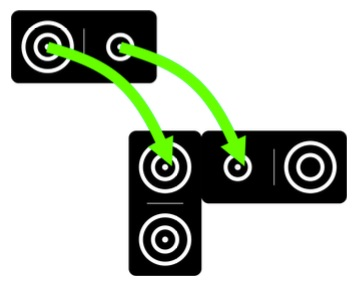
\includegraphics[scale=0.6]{climb.jpg}
\caption{Exemplo de um posicionamento a subir válido.}
\label{climb}
\end{center}
\end{figure}

Tal como no Dominó, as regras são relativamente simples. Começa-se por distribuir as peças aleatoriamente e de forma equilibrada pelos jogadores, mantendo a face voltada para baixo. 

O jogador com o duplo 7 inicia o jogo, colocando essa peça no centro da superfície de jogo e determinando a ordem dos restantes jogadores, que é dada pelo sentido contrário ao ponteiro dos relógios. 

Começando no segundo, cada jogador, na sua vez, realiza ambos os passos seguintes:
\begin{enumerate}
	\item Enquanto for possível, coloca peças a subir, podendo escolher a ordem em que o faz;
	\item Se ainda tiver alguma peça, coloca-a a expandir.
\end{enumerate}

Se, no final da sua vez, o jogador ficar sem peças, é declarado vencedor e o jogo termina. Alternativamente, os restantes jogadores podem continuar, de forma a determinar o segundo, terceiro e quarto lugares.

Na Figura~\ref{example} pode ser observado um possível jogo de Dominup a decorrer.

\begin{figure}[htbp]
\begin{center}
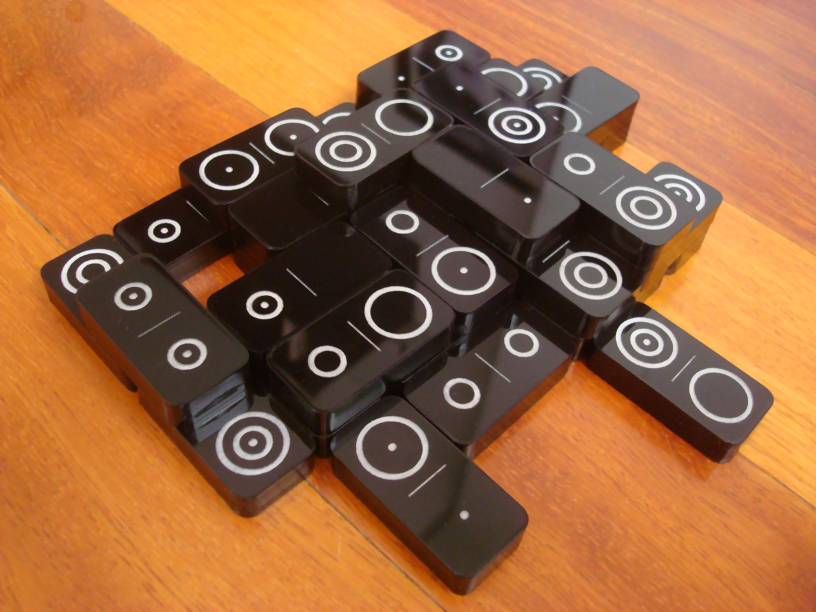
\includegraphics[scale=0.4]{example.jpg}
\caption{Exemplo de um jogo de Dominup.}
\label{example}
\end{center}
\end{figure}


%Descrever detalhadamente o jogo, a sua história e, principalmente, as suas regras.
%Devem ser incluidas imagens apropriadas para explicar o funcionamento do jogo.
%Devem ser incluidas as fontes de informação (e.g. URLs em rodapé).

%%%%%%%%%%%%%%%%%%%%%%%%%%
\section{Lógica do Jogo}

Pretendemos nas secções que se seguem descrever o projeto e implementação da lógica do jogo em Prolog, incluindo a forma de representação do estado do tabuleiro e sua visualização, a execução de movimentos, verificação do cumprimento das regras do jogo, determinação do final do jogo e cálculo das jogadas a realizar pelo computador, utilizando diversos níveis de inteligência. 

\subsection{Representação do Estado do Jogo} 

O tabuleiro de jogo no Dominup é um quadriculado, cujo tamanho não deve limitar o posicionamento de peças a expandir. Uma vez que expansões sucessivas têm que ser feitas ortogonalmente, uma linha expansiva numa só direção ocupa $2 + 1 + 2 + 1 + \cdots$ quadrículas, assumindo que a primeira peça está colocada horizontalmente. Ao todo temos 36 peças, por isso seriam necessárias $2 * 18 + 18 = 54$ quadrículas para acomodar uma tal linha de expansão. Dado que a primeira peça é colocada no centro do tabuleiro, se a expansão fosse feita sempre no mesmo sentido, poderíamos ter que considerar um tabuleiro com 108 quadrículas de lado.

Uma análise mais cuidada das regras do jogo revela que as peças são preferencialmente colocadas a subir. De facto, em cada vez, um jogador coloca tantas peças a subir quanto possível e no máximo uma peça a expandir. Além disso, em geral não será boa estratégia para nenhum dos jogadores expandir sempre no mesmo sentido. Tendo em consideração as limitações de um computador, quer em termos de capacidade de processamento, quer em termos de tamanho do ecrã, decidimos considerar um tabuleiro quadriculado de lado 18. Desta forma, é possível colocar pelo menos 5 peças em cada um dos 4 sentidos a partir do centro do tabuleiro. A experiência revela que este tamanho por vezes se torna limitativo. No entanto, tamanhos superiores entram em desacordo com o nosso princípio de manter uma apresentação visual intuitiva e agradável.

Inicialmente, o tabuleiro era representado por uma lista \verb|board| de linhas do tabuleiro. Por sua vez, cada linha é uma lista de elementos, um para cada quadrícula. Rapidamente nos apercebemos que dado o tamanho do tabuleiro esta solução não seria nada eficiente, além de que se tornava bastante complexa. Adicionalmente, o jogo que pretendíamos implementar apresenta a facilidade de ser essencialmente construtivo, as peças são colocadas na sua posição final, não havendo mudanças. Sendo assim, partimos para uma implementação do tabuleiro como um conjunto de factos do tipo 
\begin{center}
	\verb|halfPiece(Line, Column, Level, Number, Cardinal)|,
\end{center} 
representando a meia peça de dominó lá colocada, com o seguinte significado:
\begin{itemize}
	\item \verb|Line| é o linha do tabuleiro;
	\item \verb|Column| é a coluna do tabuleiro;
	\item \verb|Level| é o nível do tabuleiro em que a peça está colocada, 1 se for colocada em cima do tabuleiro, 2 se for colocada em cima dessa, etc;
	\item \verb|Number| é o número da meia peça;
	\item \verb|Cardinal| é o ponto cardeal que indica a posição da outra metade da peça (n, e, s, w).
\end{itemize}
Assim, numa quadrícula não temos qualquer predicado do tipo \verb|halfPiece|. Quando é colocado o dominó duplo 7 no meio do tabuleiro, teremos \verb|halfPiece(9, 9, 1, 7, e)| e \verb|halfPiece(9, 10, 1, 7, w)|. Numa fase mais avançada pode ser colocado o dominó $2 \cdot 6$ no nível 3 com o 2 abaixo do 6, usando os factos \verb|halfPiece(4, 5, 3, 2, n)| e \verb|halfPiece(3, 5, 3, 6, s)|.

Além do tabuleiro, o estado de jogo contém as peças de cada jogador. Dado que apenas consideramos dois jogadores nesta implementação, temos factos do tipo 
\begin{center}
\verb|piece(Number1, Number2, Player, Played)|, 
\end{center} 
com o seguinte significado:
\begin{itemize}
	\item \verb|Number1| é o menor número da peça;
	\item \verb|Number2| é o maior número da peça;
	\item \verb|Player| é 1 ou 2 consoante a peça pertença ao jogador 1 ou 2;
	\item \verb|Played| é 0, se a peça ainda não foi jogada, e 1, caso contrário.
\end{itemize}
À medida que vão sendo colocadas no tabuleiro, as peças passam a ter o indicador \verb|Played| a 1, ou seja, para cada peça jogada é revogado o facto que a representa e adicionado um novo facto, desta vez com \verb|Played| a 1.

Finalmente, o estado de jogo tem indicação de qual é o próximo jogador a jogar no facto \verb|turn(Number)|, em que number pode ser 1 ou 2.

\begin{figure}[htbp]
\begin{center}
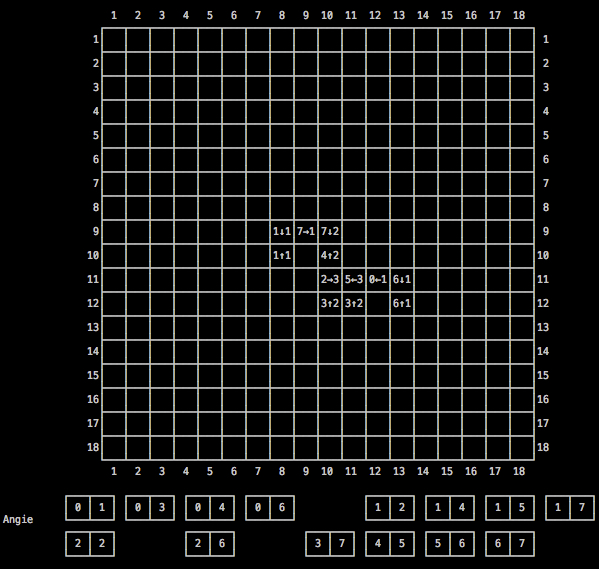
\includegraphics[scale=0.7]{intermediate.jpg}
\caption{Estado intermédio do jogo.}
\label{intermediate}
\end{center}
\end{figure}

Após algumas jogadas, podemos chegar ao estado ilustrado pela Figura~\ref{intermediate}. Em baixo estão as peças do jogador 1, dado que esse é o próximo a jogar. Em cima está o tabuleiro com as peças que contém até então. Cada meia peça colocada no tabuleiro tem do lado esquerdo o seu número e do lado direito o nível em que se encontra. Este estado é obtido com o código apresentado de seguida.


\begin{lstlisting}
/* fixed distribution of pieces used in test phase */	
testDistribute :-
        assert(piece(0, 1, 1, 0)) ,
        assert(piece(0, 3, 1, 0)) , 
        assert(piece(0, 4, 1, 0)) , 
        assert(piece(0, 6, 1, 0)) , 
        assert(piece(1, 1, 1, 0)) , 
        assert(piece(1, 2, 1, 0)) , 
        assert(piece(1, 4, 1, 0)) , 
        assert(piece(1, 5, 1, 0)) , 
        assert(piece(1, 7, 1, 0)) , 
        assert(piece(2, 2, 1, 0)) , 
        assert(piece(2, 3, 1, 0)) , 
        assert(piece(2, 6, 1, 0)) , 
        assert(piece(3, 3, 1, 0)) , 
        assert(piece(3, 7, 1, 0)) , 
        assert(piece(4, 5, 1, 0)) , 
        assert(piece(5, 6, 1, 0)) , 
        assert(piece(6, 7, 1, 0)) ,
        assert(piece(7, 7, 1, 0)) ,
        assert(piece(0, 0, 2, 0)) ,
        assert(piece(0, 2, 2, 0)) , 
        assert(piece(0, 5, 2, 0)) , 
        assert(piece(0, 7, 2, 0)) , 
        assert(piece(1, 3, 2, 0)) , 
        assert(piece(1, 6, 2, 0)) , 
        assert(piece(2, 4, 2, 0)) , 
        assert(piece(2, 5, 2, 0)) , 
        assert(piece(2, 7, 2, 0)) , 
        assert(piece(3, 4, 2, 0)) , 
        assert(piece(3, 5, 2, 0)) , 
        assert(piece(3, 6, 2, 0)) , 
        assert(piece(4, 4, 2, 0)) , 
        assert(piece(4, 6, 2, 0)) , 
        assert(piece(4, 7, 2, 0)) , 
        assert(piece(5, 5, 2, 0)) , 
        assert(piece(5, 7, 2, 0)) , 
        assert(piece(6, 6, 2, 0)) .

/* fixed plays to used in test phase */
testPlay :- playFirstPiece ,
        playPiece(2, 4, 2, 11, 10, n, _) ,
        playPiece(3, 3, 1, 12, 10, e, _) ,
        playPiece(4, 7, 2, 10, 10, n, _) ,
        playPiece(0, 5, 2, 11, 12, w, _) ,
        playPiece(2, 3, 1, 11, 10, s, _) ,
        playPiece(1, 1, 1, 9, 8, s, _) ,
        playPiece(3, 5, 2, 12, 11, n, _) ,
        playPiece(2, 5, 2, 11, 10, e, _) ,
        playPiece(6, 6, 2, 11, 13, s, _) .

/* fixed game start with distribution and plays used in test phase */
test :- 
        testDistribute , 
        testPlay , 
        assert(player(1, 'Angie', 1)) , 
        assert(player(2, 'Nuno', 1)).
\end{lstlisting}

Um possível estado final, tem a ilustração da Figura~\ref{over}, onde se pode observar, além do tabuleiro, o jogador que venceu.

\begin{figure}[htbp]
\begin{center}
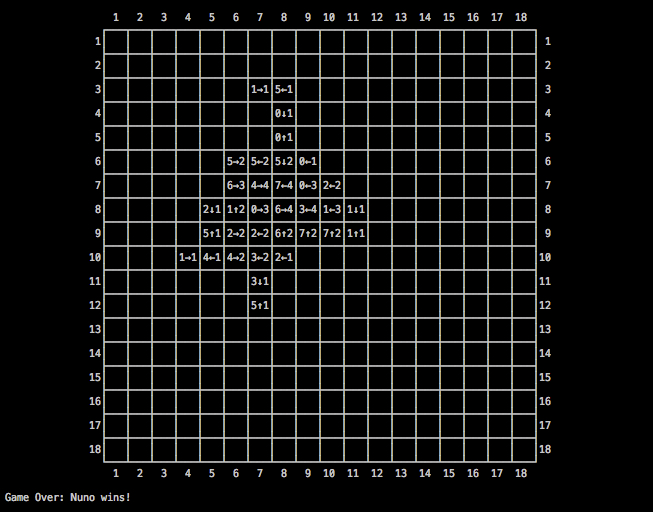
\includegraphics[scale=0.6]{final.jpg}
\caption{Estado final do jogo.}
\label{over}
\end{center}
\end{figure}

%Descrever a forma de representação do estado do tabuleiro (tipicamente uma lista de listas), com exemplificação em Prolog de posições iniciais do jogo, posições intermédias e finais, acompanhadas de imagens ilustrativas.

\subsection{Visualização do Tabuleiro}
 
Para visualizar o tabuleiro em modo de texto, cada quadrícula é sempre desenhada com traços a toda a volta, independentemente da posição das peças. Cada peça é colocada em duas quadrículas adjacentes e a relação entre as duas metades é identificada pelo conteúdo das células. Isto é, o dominó~$2 \cdot 5$ dá origem às células \verb|2→3| e \verb|5←3|, se for colocado no nível 3 na horizontal com o 2 à esquerda do 5. O resultado é aquele que se pode observar nas Figuras~\ref{intermediate} e~\ref{over}.

Os predicados usados para este efeito cuja definição pode ser consultada no Anexo~\ref{codigo} são os seguintes:
\begin{itemize}
	\item \verb|printBoard| - para imprimir o tabuleiro de jogo;
	\item \verb|printRows| - para imprimir as linhas do tabuleiro;
	\item \verb|printCells| - para imprimir as quadrículas do tabuleiro;
	\item \verb|getTopLevel(X, Y, L)| - para obter o nível mais elevado de uma quadrícula;
	\item \verb|printCardinal| - para imprimir o cardeal (n, e, s, w) usando setas;
	\item \verb|printNumbers| - para imprimir os números no topo e no fim do tabuleiro;
	\item \verb|printLeftNumbers(X)| - para imprimir o número à esquerda da linha X do tabuleiro;
	\item \verb|printRightNumbers(X)| - para imprimir o número à direita da linha X do tabuleiro;
	\item \verb|printGridTop| - para imprimir o topo da grelha do tabuleiro;
	\item \verb|printGrid(X)| - para imprimir a linha X da grelha do tabuleiro;
	\item \verb|printSpaces(N)| - para imprimir N espaços;
	\item \verb|printPlayerName(I)| - para imprimir o nome do jogador I usando exatamente N caracteres;
	\item \verb|printPlayer(I)| - para imprimir o jogador I;
	\item \verb|printPieces(I, C, R, N1T, N2T, N1N, N2N, N1B, N2B)| - para imprimir o nome e as peças do jogador I, todos os restantes argumentos começam em 0;
	\item \verb|printPieceTop(P)| - para imprimir o rebordo do topo da peça, onde P indica se já foi jogada ou não;
	\item \verb|printPieceNumber(P)| - para imprimir os números da peça, onde P indica se já foi jogada ou não;
	\item \verb|printPieceBottom(P)| - para imprimir o rebordo do fundo da peça, onde P indica se já foi jogada ou não;
	\item \verb|printGame(I)| - para imprimir o jogo, de forma que o jogador I possa jogar na sua vez;
	\item \verb|printGameOver(I)| - para imprimir o estado final do jogo, quando venceu o jogador I.
\end{itemize}

\subsection{Lista de Jogadas Válidas} 

Uma vez que no Dominup há dois tipos distintos de movimentos, subir e expandir, usamos duas listas de jogadas válidas. Estas listas são usadas por ambas as inteligências artificiais para decidir os seus próximos movimentos.

Para obter estas listas são usados os predicados que se apresentam de seguida.

\begin{lstlisting}
/* predicate used to check if a climb movement is valid */
/* this is very similar to checkPlay above, but only for climbs, and works with findall */
checkClimb(N1, N2, I, X1, Y1, C1) :-                            
        checkPlayerPiece(N1, N2, I) ,                           /* check if the piece belongs to the player and has not been played */
        getTopLevel(X1, Y1, L) ,                                /* obtain the current level of the position on the board */
        getOtherHalf(X1, Y1, C1, X2, Y2, _) ,                   /* obtain the position of the other half of the piece */
        checkInsideBoard(X1, Y1, X2, Y2) ,                      /* verify that the whole piece is inside the board */
        checkLevelStable(L, X2, Y2) ,                           /* verify that the level of both halfs is the same */
        checkClimbNumbers(N1, X1, Y1, N2, X2, Y2, L).           /* check that the numbers are correct for climbing */

/* predicate used to check if an expand movement is valid */
/* this is very similar to checkPlay above, but only for expand, and works with findall */
checkExpand(N1, N2, I, X1, Y1, C1) :- 
        checkPlayerPiece(N1, N2, I) ,                           /* check if the piece belongs to the player and has not been played */
        position(X1, Y1),                                       /* verify that X1, Y1 is a valid board position */
        getOtherHalf(X1, Y1, C1, X2, Y2, C2) ,                  /* obtain the position of the other half of the piece */ 
        checkInsideBoard(X1, Y1, X2, Y2) ,                      /* verify that the whole piece is inside the board */    
        checkLevelStable(0, X1, Y1),                            /* verify that the level of both halfs is the 0 */    
        checkLevelStable(0, X2, Y2) , 
        checkExpandOrthogonal(X1, Y1, C1, X2, Y2, C2).          /* check that there is some other piece on the board orthogonal to this one */

/* predicate used to obtain a list of all possible climb movements for a player */
getClimbPlays(I, Plays) :- 
        findall(play(N1, N2, I, X1, Y1, C1), checkClimb(N1, N2, I, X1, Y1, C1), Plays).

/* predicate used to obtain a list of all possible expand movements for a player */
getExpandPlays(I, Plays) :- 
        findall(play(N1, N2, I, X1, Y1, C1), checkExpand(N1, N2, I, X1, Y1, C1), Plays).
\end{lstlisting}

Estes predicados invocam outros que não estão aqui representados, mas os seus nomes e comentários são elucidativos. De qualquer forma, a sua definição está no Anexo~\ref{codigo} e na secção seguinte.

\subsection{Execução de Jogadas} 

Sempre que o jogador humano indica um novo movimento este é validado e, em caso de sucesso, a peça é jogada. Para isso usam-se os predicados seguintes:

\begin{lstlisting}
/* predicate used to play a piece */
playPiece(N1, N2, I, X1, Y1, C1, L) :-                          /* L is output */
        checkPlay(N1, N2, I, X1, Y1, C1, X2, Y2, C2, L) ->      /* check if this play is valid */
        (L1 is L + 1 ,                                          /* the new level is 1 above the current level */
         assert(halfPiece(X1, Y1, L1, N1, C1)) ,                /* create first halfPiece */
         assert(halfPiece(X2, Y2, L1, N2, C2)) ,                /* create second halfPiece */
         retract(piece(N1, N2, I, 0)) ,                         /* remove piece from player's hand */
         assert(piece(N1, N2, I, 1))) ;                         /* place piece back but marked as played */
        fail.                                                   /* if checkPlay fails, fail and do nothing */

/* predicate used to check if a play is valid */
checkPlay(N1, N2, I, X1, Y1, C1, X2, Y2, C2, L) :-              /* X2, Y2, C2 and L are output */
        getTopLevel(X1, Y1, L) ,                                /* find the current level of the position X1, Y1 */
        getOtherHalf(X1, Y1, C1, X2, Y2, C2) ,                  /* compute the position of the other half given X1, Y1 and C1 */
        checkInsideBoard(X1, Y1, X2, Y2) ,                      /* verify that the piece will be place inside the board */
        checkPlayerPiece(N1, N2, I) ,                           /* verify that the player holds the piece and it has not been played yet */
        checkLevelStable(L, X2, Y2) ,                           /* verify that the other half has the same level */
        (L == 0 ->                                              /* if the current level is 0 */
         checkNoClimbs(I) ,                                     /* verify that the player has no more climb moves */
         checkExpandOrthogonal(X1, Y1, C1, X2, Y2, C2) ;        /* and check that this expansion is orthogonal to another piece on the board */
         checkClimbNumbers(N1, X1, Y1, N2, X2, Y2, L)).         /* otherwise verify that the climb is on correct numbers */

/* predicate used to check if the piece is inside the board */
checkInsideBoard(X1, Y1, X2, Y2) :- 
        check1InsideBoard(X1) ,                                 /* simply check each coordinate */
        check1InsideBoard(Y1) , 
        check1InsideBoard(X2) , 
        check1InsideBoard(Y2).

/* predicate used to check if a given coordinate is inside the board */
check1InsideBoard(Z) :- Z < 1 -> fail ; (Z > 18 -> fail ; true).

/* predicate used to check if the piece belongs to the player and has not been played */
checkPlayerPiece(N1, N2, I) :- piece(N1, N2, I, 0).

/* predicate used to check if the other half has the same level */
checkLevelStable(L, X2, Y2) :- getTopLevel(X2, Y2, L).

/* predicate used to check if the numbers for a climb placement are correct */
checkClimbNumbers(N1, X1, Y1, N2, X2, Y2, L) :- halfPiece(X1, Y1, L, N1, _) , halfPiece(X2, Y2, L, N2, _).

/* predicate used to check if the expand placement is orthogonal to some piece on the board */
checkExpandOrthogonal(X1, Y1, C1, X2, Y2, C2) :- 
        checkHalfOrthogonal(X1, Y1, C1) ;                       /* succeeds if at least one half has an orthogonal piece */
        checkHalfOrthogonal(X2, Y2, C2).

/* predicate used to check if a piece half has an orthogonal on the board */
checkHalfOrthogonal(X, Y, C) :- 
        checkNorthOrthogonal(X, Y, C) ;                         /* succeeds if at least one cardinal has an orthogonal piece*/
        checkEastOrthogonal(X, Y, C) ; 
        checkSouthOrthogonal(X, Y, C) ; 
        checkWestOrthogonal(X, Y, C).

/* predicate used to check if a piece half has an orthogonal on the North */
checkNorthOrthogonal(X, Y, C) :-
        X1 is X - 1 ,                                           /* North line is this line minus 1 */
        (member(C, [e, w]) ->                                   /* if C is East or West */
         halfPiece(X1, Y, 1, _, n) ;                            /* North half piece must have cardinal North */
         (C == s ->                                             /* alternatively, if C is South */
          (halfPiece(X1, Y, 1, _, e) ;                          /* North half piece can have cardinal East */
           halfPiece(X1, Y, 1, _, w))                           /* or West */
         ; fail)).                                              /* in all other cases, fail */

/* predicate used to check if a piece half has an orthogonal on the East */
checkEastOrthogonal(X, Y, C) :-                                 /* very similar to North case */
        Y1 is Y + 1 , 
        (member(C, [s, n]) -> 
         halfPiece(X, Y1, 1, _, e) ;
         (C == w -> 
          (halfPiece(X, Y1, 1, _, n) ; 
           halfPiece(X, Y1, 1, _, s)) ; 
          fail)).

/* predicate used to check if a piece half has an orthogonal on the South */
checkSouthOrthogonal(X, Y, C) :-                                /* very similar to North case */
        X1 is X + 1 , 
        (member(C, [w, e]) -> 
         halfPiece(X1, Y, 1, _, s) ;
         (C == n -> 
          (halfPiece(X1, Y, 1, _, e) ; 
           halfPiece(X1, Y, 1, _, w)) ; 
          fail)).

/* predicate used to check if a piece half has an orthogonal on the West */
checkWestOrthogonal(X, Y, C) :-                                 /* very similar to North case */
        Y1 is Y - 1 , 
        (member(C, [n, s]) -> 
         halfPiece(X, Y1, 1, _, w) ;
         (C == e -> 
          (halfPiece(X, Y1, 1, _, n) ; 
           halfPiece(X, Y1, 1, _, s)) ; 
          fail)).

/* predicate used to check if a player has no more climb moves */
checkNoClimbs(I) :-                                             
        getClimbPlays(I, Plays) ,                               /* compute all climb plays for player */
        length(Plays, Number) ,                                 /* obtain the number of climb plays */
        Number == 0.                                            /* if it is 0, there are no more climb plays */
\end{lstlisting}


\subsection{Avaliação do Tabuleiro}

A inteligência artificial mais complexa necessita de avaliar o estado do jogo a cada passo para decidir como prosseguir. Uma vez que o estado de jogo é um conjunto de factos, para fazer esta avaliação, é jogada uma das peças possíveis, depois o estado é avaliado e a peça é retirada do tabuleiro. Note-se que é necessário fazer isto para todas as jogadas possíveis, de forma a escolher a que apresenta melhor avaliação. Tudo isto é feito com os predicados abaixo.

\begin{lstlisting}
/* predicate used to evaluate the current situation of the game for a given player */
evaluateSituation(I, R) :-                                      /* R is the result, bigger R means better for player I */
        getNumberPlays(I, Rme) ,                                /* compute the number of pieces player I can play */
        I1 is 3 - I ,                                           /* I1 is the other player */
        getNumberPlays(I1 , Ryou) ,                             /* compute the number of pieces the other player can play */
        R is Rme - Ryou.                                        /* the result is the difference */

/* predicate used to compute the maximum number of plays for a given player*/
getNumberPlays(I, R) :- 
        getClimbPlays(I, Plays),                                /* get list of all climbs */
        length(Plays, S) ,                                      /* compute maximum number of climbs */
        R is S + 1.                                             /* the result is the number of climbs plus 1, because there is always 1 expand */

/* predicate used to play a piece without checking it is valid */
playPieceNoCheck(N1, N2, I, X1, Y1, C1, L) :-                   /* very similar to playPiece, but faster */
        getOtherHalf(X1, Y1, C1, X2, Y2, C2) , 
        getTopLevel(X1, Y1, L) , L1 is L + 1 , 
        assert(halfPiece(X1, Y1, L1, N1, C1)) , 
        assert(halfPiece(X2, Y2, L1, N2, C2)) , 
        retract(piece(N1, N2, I, 0)) , 
        assert(piece(N1, N2, I, 1)).

/* predicate used to remove a piece from the board */
removePiece(N1, N2, I, X1, Y1, C1, L) :-                        /* does the opposite of playPieceNoCheck */
        getOtherHalf(X1, Y1, C1, X2, Y2, C2) , 
        getTopLevel(X1, Y1, L) , 
        retract(halfPiece(X1, Y1, L, N1, C1)) , 
        retract(halfPiece(X2, Y2, L, N2, C2)) , 
        assert(piece(N1, N2, I, 0)) , 
        retract(piece(N1, N2, I, 1)).

/* predicate used to evaluate how good a given climb is */
evaluateClimb(N1, N2, I, X1, Y1, C1, R) :-                      /* R is the result, bigger R means better climb */
        checkClimb(N1, N2, I, X1, Y1, C1) ,                     /* first check if the climb is valid */
        playPieceNoCheck(N1, N2, I, X1, Y1, C1, _) ,            /* then play it */
        evaluateSituation(I, R) ,                               /* then evaluate the current situation */
        removePiece(N1, N2, I, X1, Y1, C1, _).                  /* then remove the played piece */

/* predicate used to evaluate how good a given expand is */
evaluateExpand(N1, N2, I, X1, Y1, C1, R) :-                     /* very similar to evaluateClimb */
        checkExpand(N1, N2, I, X1, Y1, C1) , 
        playPieceNoCheck(N1, N2, I, X1, Y1, C1, _) , 
        evaluateSituation(I, R) , 
        removePiece(N1, N2, I, X1, Y1, C1, _).

/* predicate used to obtain a list of all climb plays evaluated */
evaluateClimbPlays(I, Plays) :- 
        findall(play(N1, N2, I, X1, Y1, C1, R), evaluateClimb(N1, N2, I, X1, Y1, C1, R), Plays).

/* predicate used to obtain a list of all expand plays evaluated */
evaluateExpandPlays(I, Plays) :- 
        findall(play(N1, N2, I, X1, Y1, C1, R), evaluateExpand(N1, N2, I, X1, Y1, C1, R), Plays).
\end{lstlisting}

\subsection{Final do Jogo}

A cada passo do jogo, é verificado se este terminou, o que acontece quando um dos jogadores ficar sem peças. Esta avaliação é feita pelo seguinte predicado em Prolog:

\begin{lstlisting}
/* predicate used to check if the game is over */
checkGameOver :-                                                /* the name is misleading, fails if game over, succeeds otherwise */
        numberPieces(1, 0, 0, 0, R1) ,                          /* get number of pieces of player 1 */
        (R1 == 0 ->                                             /* if player 1 has 0 pieces */
         (printGameOver(1), fail) ;                             /* player 1 has won, print that and fail */
         (numberPieces(2, 0, 0, 0, R2),                         /* otherwise, get number of pieces of player 2 */      
          (R2 == 0 ->                                           /* if player 2 has 0 pieces */   
           (printGameOver(2) , fail) ;                          /* player 2 has won, print that and fail */ 
           true))).                                             /* otherwise the game continues */
\end{lstlisting}

\subsection{Jogada do Computador} 

A jogada do computador é feita consoante o nível de inteligência. Isto é verificado durante a vez do jogador, dado o seu tipo. De facto, em caso de jogador humano (tipo 1), o motor de jogo invoca os predicados que pedem ao utilizador para indicar a jogada e que a executam; em caso de jogador do tipo computador fácil, é invocado o predicado \verb|playRandom|, que faz uma sequência de jogadas aleatórias; em caso de jogador do tipo computador difícil, é invocado o predicado \verb|playBest|, que faz uma sequência de jogadas em modo ganancioso, isto é, escolhendo sempre uma das que lhe parecem melhores. A definição destes predicados é a seguinte:

\begin{lstlisting}
/* predicate used play a random climb movement */
randomClimbPlay(I) :- 
        getClimbPlays(I, Plays) , 
        random_member(play(N1, N2, I, X1, Y1, C1), Plays) , 
        playPiece(N1, N2, I, X1, Y1, C1, _).

/* predicate used play a random expand movement */
randomExpandPlay(I) :- 
        getExpandPlays(I, Plays) , 
        random_member(play(N1, N2, I, X1, Y1, C1), Plays) , 
        playPiece(N1, N2, I, X1, Y1, C1, _).

/* predicate used play a random turn */
playRandom(I) :- 
        randomClimbPlay(I) ->                                   /* while there are valid climbs */
        playRandom(I) ;                                         /* do random climbs */
        randomExpandPlay(I).                                    /* afterward do one expand */

/* predicate used to play one of the best climb plays available */
bestClimbPlay(I) :- 
        evaluateClimbPlays(I, Plays) , 
        bestPlay(Plays, play(N1, N2, I, X1, Y1, C1, _)) , 
        playPiece(N1, N2, I, X1, Y1, C1, _).

/* predicate used to play one of the best expand plays available */
/* since there are usually many expand plays available, this is the slowest function taking a few seconds to finish */
bestExpandPlay(I) :- 
        evaluateExpandPlays(I, Plays) , 
        bestPlay(Plays, play(N1, N2, I, X1, Y1, C1, _)) , 
        playPiece(N1, N2, I, X1, Y1, C1, _).

/* predicate used play a greedy turn, always choosing one of the best available plays */
playBest(I) :- bestClimbPlay(I) -> playBest(I) ; bestExpandPlay(I).
\end{lstlisting}

%%%%%%%%%%%%%%%%%%%%%%%%%%
\section{Interface com o Utilizador}

O utilizador apenas necessita de ir digitando alguns caracteres no teclado, seguidos da tecla Enter, interagindo dessa forma com o jogo.

\begin{figure}[htbp]
\begin{center}
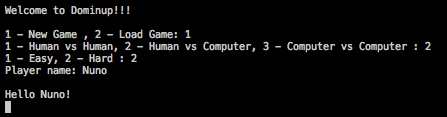
\includegraphics[scale=0.6]{input_ini.jpg}
\caption{Interface inicial do jogo}
\label{input_ini}
\end{center}
\end{figure}

No ecrã inicial o jogador tem de escolher se pretende iniciar um novo jogo ou um previamente gravado. Se escolher um jogo já gravado, este é carregado com as definições inicialmente selecionadas pelo utilizador e o jogo continuará a se desenrolar. Caso contrário, o jogador tem de escolher se pretende jogar contra o computador, contra outro jogador ou observar um jogo entre dois computadores. 

Sendo o nível de dificuldade, fácil ou difícil, escolhido logo a seguir, para terminar a configuração do jogo falta apenas escrever o(s) nome(s) do(s) jogador(es). A Figura~\ref{input_ini} ilustra o interface inicial com o utilizador.

O jogo inicia mostrando o tabuleiro de jogo com a peça duplo 7 colocada no meio do tabuleiro. O jogador que tem a vez é aquele que não tinha essa peça, dado que o outro já jogou o duplo 7 como obrigam as regras. Para jogar, cada jogador tem acesso às suas peças e é convidado a escolher o movimento para realizar uma jogada. Para tal deve indicar o seguinte:

\begin{itemize}
\item colocar o número do lado esquerdo da peça que pretende jogar;
\item colocar o número da lado direito da peça que pretende jogar;
\item indicar onde pretende colocar a metade esquerda da peça, indicando para isso a linha e a coluna;
\item indicar a orientação da peça, dizendo para isso onde se situa a metade direita da peça em relação à metade esquerda, utilizando as opções n, e, s e w, designando norte, este, sul e oeste, respetivamente.
\end{itemize}

Em lugar de escolher um movimento, o jogador pode também indicar que pretende salvar o jogo e sair. A Figura~\ref{input_mid} ilustra o interface com o utilizador durante o jogo.

\begin{figure}[htbp]
\begin{center}
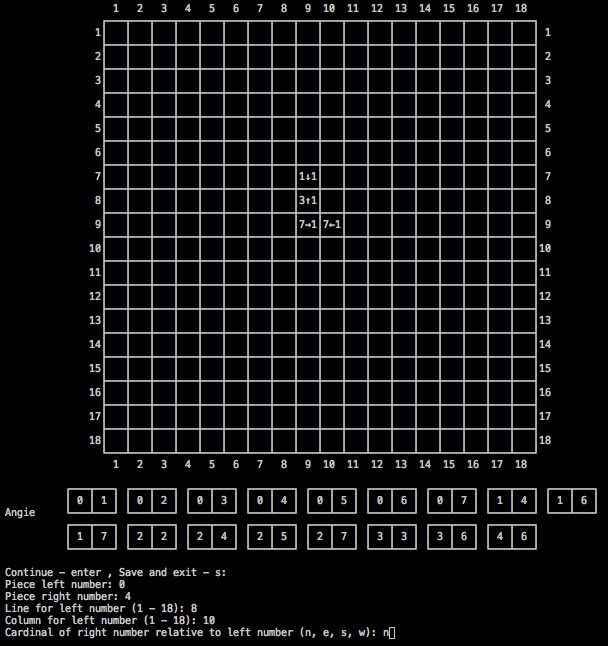
\includegraphics[scale=0.5]{input_mid.jpg}
\caption{Interface de uma jogada}
\label{input_mid}
\end{center}
\end{figure}


%%%%%%%%%%%%%%%%%%%%%%%%%%
\section{Conclusões}

Este jogo foi desde logo uma das nossas primeiras hipóteses de seleção, de entre quatro possíveis, para se desenvolver o primeiro projeto em Prolog que seria objeto de avaliação. Ficamos extremamente felizes com o desenvolvimento de um jogo que à partida trazia alguma nostalgia pelo simples facto de nos lembrar alguns momentos, em que outrora um simples jogo de Dominó fazia a delícia dos mais pequenos. 

Somos da opinião que este jogo trás uma espécie de reformulação do típico jogo de dominó e que faz todo o sentido coloca-lo disponível a jogar num computador, apesar de ainda em modo de texto.

Relativamente ao projeto consideramos que tudo o que delineamos e que todos os pontos exigidos na implementação do jogo foram cumpridos. Foi muito proveitoso uma vez que serviu também para praticarmos e aumentarmos a nossa prática em programação lógica.

Gostaríamos de ter desenvolvido mais um nível de inteligência artificial. De momento o nível difícil não avalia como as jogadas do adversário podem afetar os planos do computador, por exemplo. Também queríamos ter colocado a dimensão do tabuleiro de jogo a ser adaptada dinamicamente, isto é, consoante a colocação de peças e os movimentos de expansão, o tabuleiro ir aumentando de dimensão.

Todavia, estamos agradados com o rumo que o projeto tomou e o resultado final foi o que esperávamos.


\clearpage
\section{Bibliografia}
\begin{itemize}
	\item http://www.nestorgames.com
	\item https://sicstus.sics.se/sicstus/docs/4.0.3/html/sicstus/Saving.html
	\item https://sicstus.sics.se/sicstus/docs/latest4/pdf/sicstus.pdf
	\item Apontamentos das aulas teóricas
\end{itemize}

\newpage
\appendix
\section{Código fonte do jogo Dominup em Prolog}
\label{codigo}

Apresenta-se a seguir todo o código fonte utilizado no projeto. Como não conseguimos processar os caracteres unicode para desenhar caixas na consola no \LaTeX, o código do ficheiro display.pl é ligeiramente diferente, mas apenas nos predicados que desenham a grelha do tabuleiro e as grelhas das peças.

\subsection{Ficheiro main.pl}
\lstinputlisting{main.pl}

\subsection{Ficheiro display.pl}
\lstinputlisting{display.pl}

\subsection{Ficheiro dominup.pl}
\lstinputlisting{dominup.pl}

\end{document}
